\begin{frame}[fragile,label=diminishDelay]{diminishing returns: register delays}
\begin{tikzpicture}
    \tikzset{
        logic/.style 2 args={draw,rectangle,align=center,anchor=north west,minimum width=#1,on chain,join,
                      inner sep=4pt,outer sep=1pt,minimum height=0.75cm,
                      label={[font=\small]-90:#2},fill=blue!30,font=\scriptsize},
        myl/.style 2 args={label={[align=right]180:#2 ps\\per cycle}},
        myReg/.style={hReg={10 ps},minimum height=0.75cm,on chain,join},
        every join/.style={-Latex,very thick},
        my chain/.style={start chain,node distance=5mm},
    }
    \matrix {
    \begin{scope}[my chain]
        \node[logic={5cm}{100 ps},myl={1 stage}{110}] {logic (all)};
        \node[myReg] {};
    \end{scope} \\
    \begin{scope}[my chain]
        \node[logic={2.5cm}{50 ps},myl={2 stage}{60}] {logic (1/2)};
        \node[myReg] {};
        \node[logic={2.5cm}{50 ps}] {logic (2/2)};
        \node[myReg] {};
    \end{scope} \\
    \begin{scope}[my chain]
        \node[logic={1.5cm}{33 ps},myl={5 stage}{43}] {logic (1/3)};
        \node[myReg] {};
        \node[logic={1.5cm}{33 ps}] {logic (2/3)};
        \node[myReg] {};
        \node[logic={1.5cm}{33 ps}] {logic (3/3)};
        \node[myReg] {};
    \end{scope} \\
    \begin{scope}[my chain, node distance=20mm, every node/.style={inner sep=0pt}]
        \node[on chain] {\vdots};
        \node[on chain] {\vdots};
        \node[on chain] {\vdots};
        \node[on chain] {\vdots};
    \end{scope}
    \\
    \begin{scope}[my chain,node distance=7mm]
        \node[logic={0.1cm}{1 ps},myl={100 stage}{11}] {\strut};
        \node[myReg] {};
        \node[logic={0.1cm}{1 ps}] {\strut};
        \node[myReg] {};
        \node[logic={0.1cm}{1 ps}] {\strut};
        \node[myReg] {};
        \node[logic={0.1cm}{1 ps}] {\strut};
        \node[myReg] {};
        \node[on chain,join] {\ldots};
    \end{scope} \\
    };
\end{tikzpicture}
\end{frame}

% FIXME: graph
\begin{frame}[fragile,label=regDelayLat]{diminishing returns: register delays}
\begin{tikzpicture}
\begin{axis}[width=.95\textwidth,height=0.8\textheight,xlabel={number of stages},ylabel={time per completion (ps)},
    xmin=0.5,xmax=15.5,ymin=0,ymax=120]
    \addplot[domain=1:15,samples=15,only marks,blue] {100/x+10}
        coordinate[pos=0] (t0)
        coordinate[pos=1/14] (t1)
        coordinate[pos=13/14] (t13)
        coordinate[pos=14/14] (t14);
    \path[name path=ten] (0,10) -- (16, 10);
    \path[name path=zero] (0,0) -- (16, 0);
    \only<2->{
        \addplot+[pattern=north west lines,opacity=0.2] fill between[of=ten and zero];
        \node[anchor=center] at (8,5) { register delay };
    }
    \only<3->{
        \draw[red] (t0) -| (t1) node[near start, right] {1.83x speedup};
        \draw[red] (t13) -| (t14) node[near start, above, xshift=-1cm] {1.02x speedup};
    }
\end{axis}
\end{tikzpicture}
\end{frame}

\begin{frame}[fragile,label=regDelayThru]{diminishing returns: register delays}
\begin{tikzpicture}
\begin{axis}[width=.95\textwidth,height=0.8\textheight,xlabel={number of stages},ylabel={throughput (ops/ns)},
    xmin=0.5,xmax=15.5,ymin=0,ymax=105]
    \addplot[domain=1:15,samples=15,only marks,blue] {1000/(100/x+10)}
        coordinate[pos=0] (t0)
        coordinate[pos=1/14] (t1)
        coordinate[pos=13/14] (t13)
        coordinate[pos=14/14] (t14);
    \draw[red] (t0) -| (t1) node[midway, right] {1.83x throughput};
    \draw[red] (t13) -| (t14) node[near start, above, xshift=-1.5cm] {1.02x throughput};
    \only<2->{
        \draw[red,dashed,line width=1pt] (0,100) -- (16,100)
            node[midway,below] {max. rate of register updates};
    }
\end{axis}
\end{tikzpicture}
\end{frame}

